\begin{abstract}

Our analysis of the key-value activity generated by the ParSplice molecular
dynamics simulation demonstrates the need for more complex cache management
strategies. Baseline measurements show clear keyspace access patterns and hot
spots that offer significant opportunity for optimization. We use the data
management and policy engine from the Mantle system to dynamically explore a
variety of techniques, ranging from basic algorithms and heuristics to
statistical models, calculus, and machine learning. While Mantle was originally
designed for distributed file systems, we show how the collection of
abstractions effectively decomposes the problem into manageable policies for a
different domain and service.  Our exploration of this space results in a
dynamically sized cache policy that, for our initial conditions, sacrifices
negligible performance while using only 28\% of the memory required by our
hand-tuned cache.

\end{abstract}

\section{Introduction}

The fine-grained data annotation capabilities provided by key-value storage is
a natural match for many types of scientific simulation. Simulations relying on
a mesh-based decomposition of a physical region may result in millions or
billions of mesh cells. Each cell contains materials, pressures, temperatures
and other characteristics that are required to accurately simulate phenomena of
interest. In our target application, the
ParSplice~\cite{perez:jctc20150parsplice} molecular dynamics simulation, a
hierarchy of caches and a single persistent key-value store are used to store
both observed minima across a molecule's equation of motion (EOM) and the
hundreds or thousands of partial trajectories calculated each second during a
parallel job. Unfortunately, if we scale the system the IO to the storage
hierarchy will quickly saturate both the storage and bandwidth capacity of a
single node, so we need more effective data management techniques, such as
cache management or load balancing across a cluster.

\begin{figure}[t]
\noindent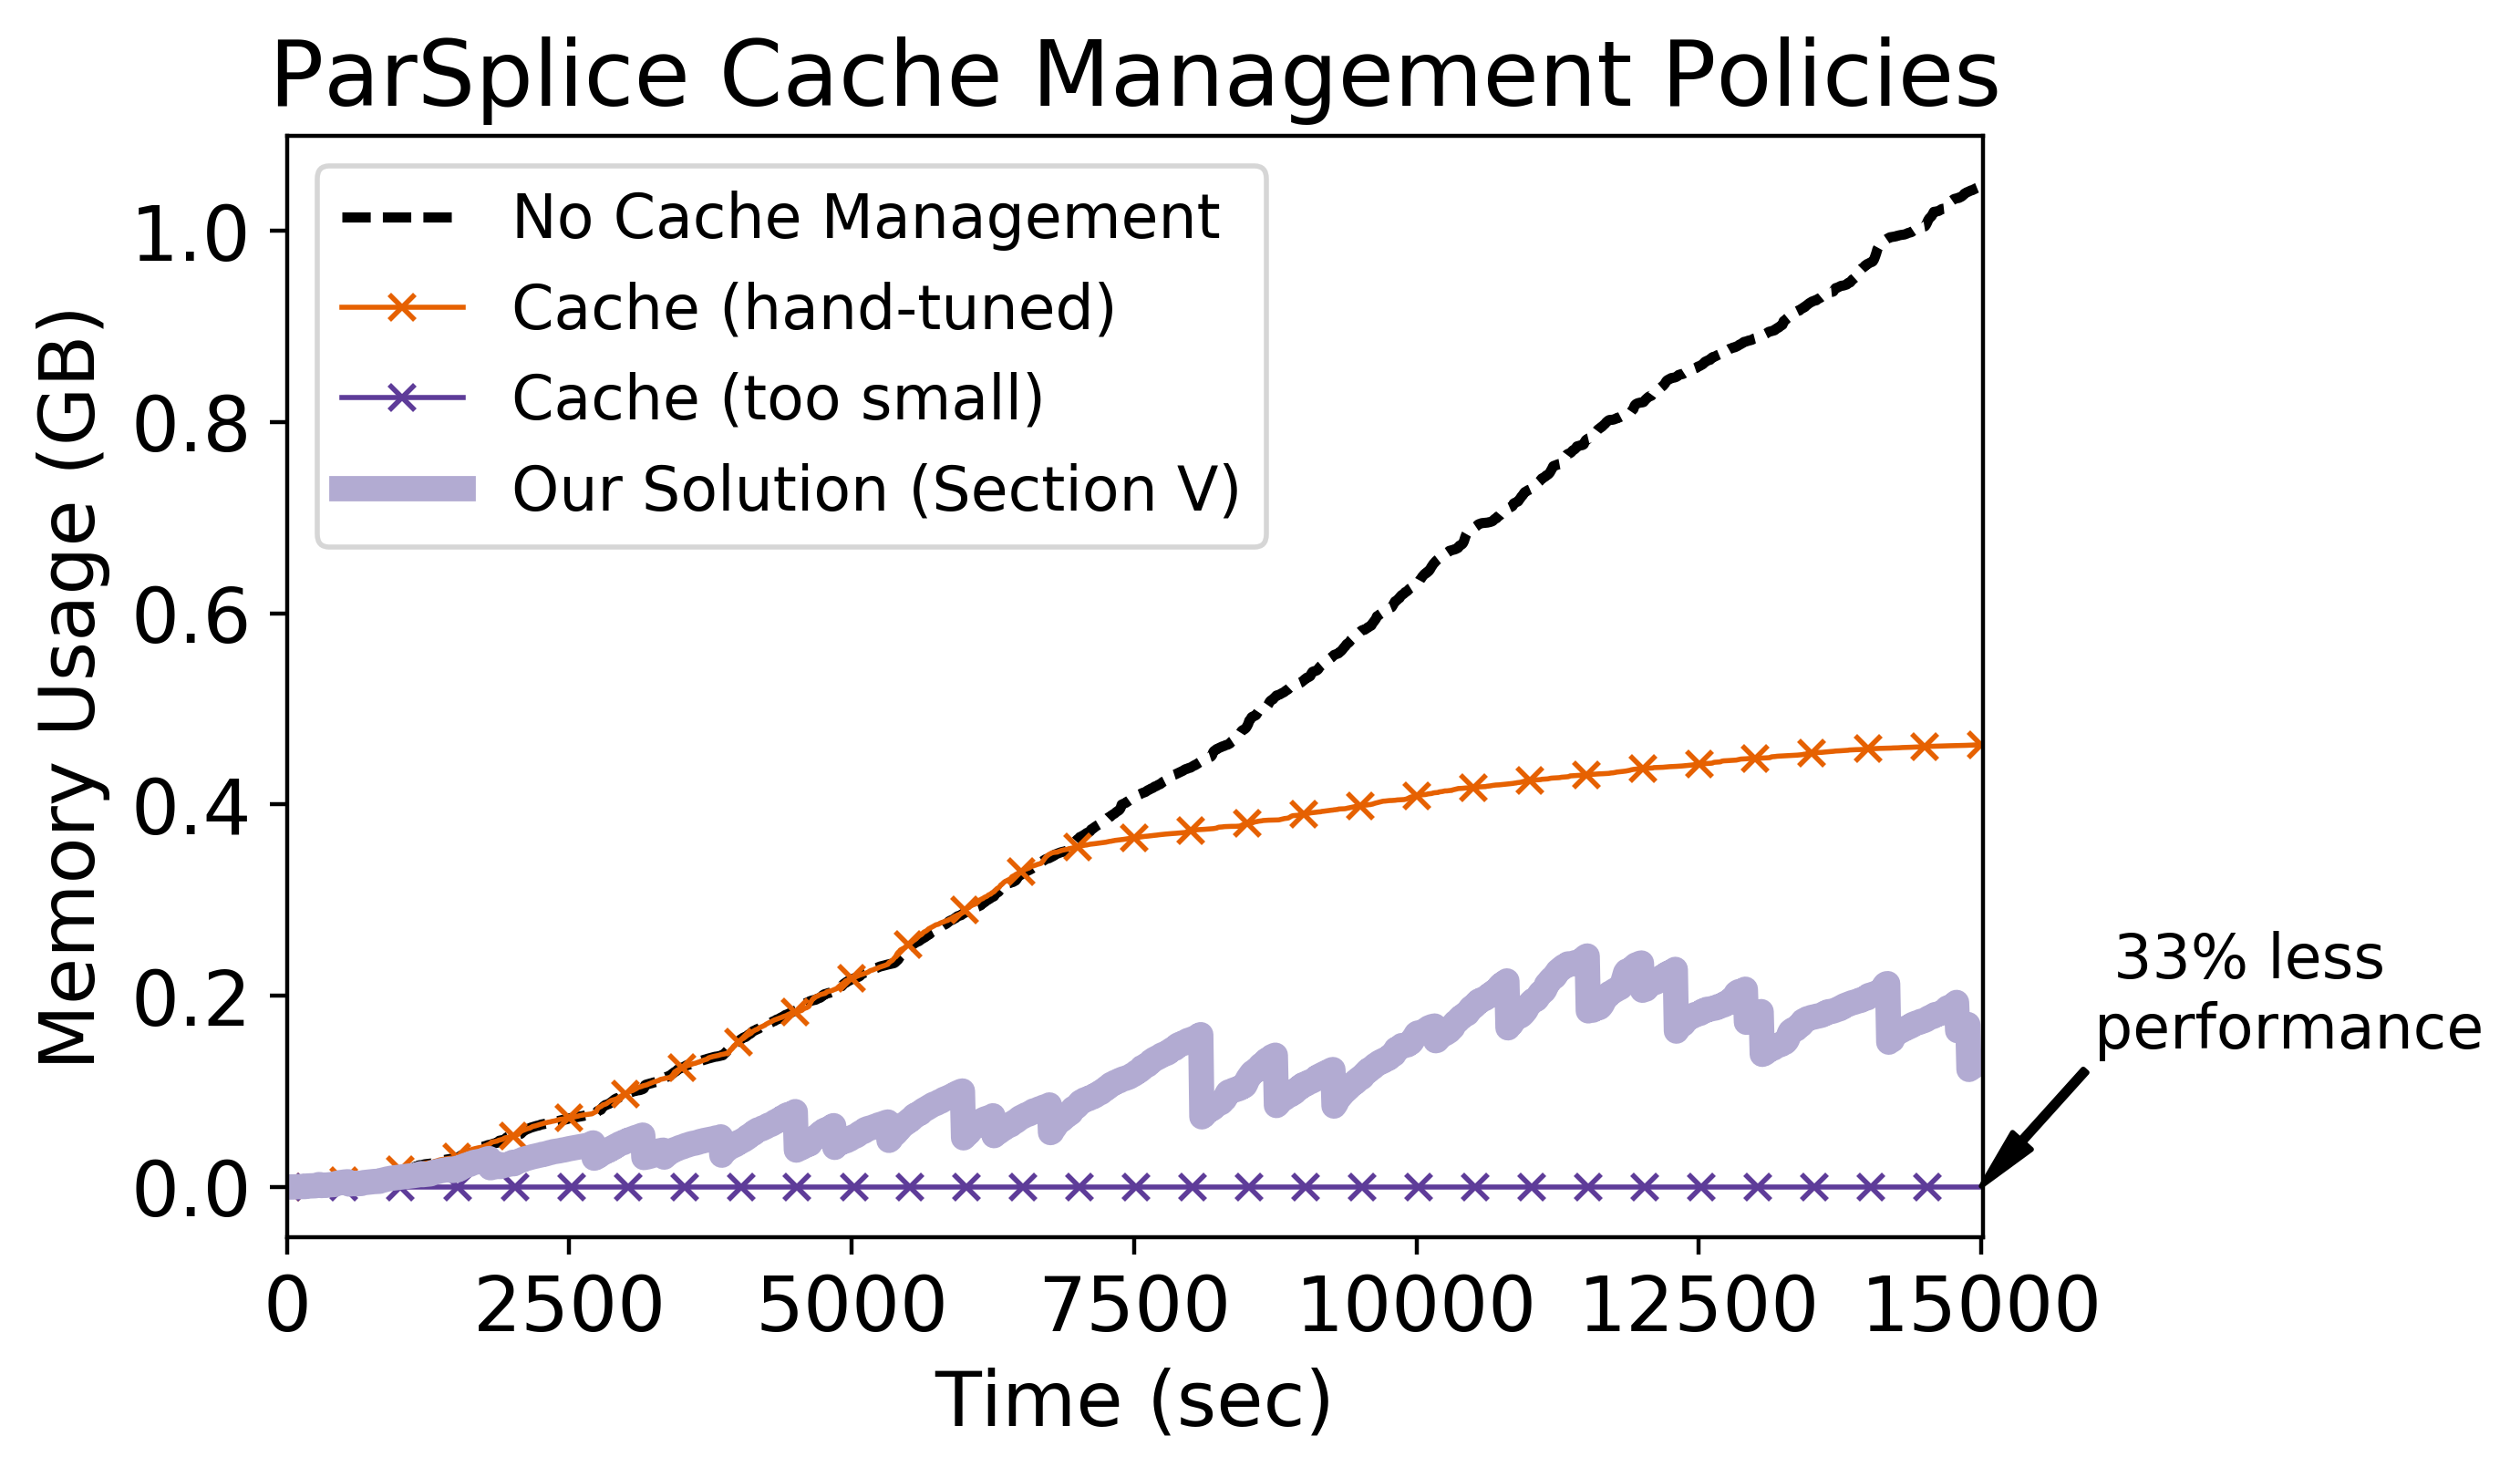
\includegraphics[width=0.5\textwidth]{figures/cache-management.png}\\

\caption{Using our data management language and Mantle policy engine, we
designed a dynamically sized caching policy for the ParSplice application. The
solution uses knowledge about the application to detect key access patterns and
adjust the cache accordingly. 
\label{fig:cache-management}}
\end{figure}

The biggest challenge for ParSplice is properly sizing the caches in the
storage hierarchy.  The memory usage for a ParSplice cache that stores molecule
coordinates is shown in Figure~\ref{fig:cache-management}. The solid lines are
the existing cache management policies, exposed as configurations in ParSplice.
The default ParSplice configuration uses an unlimited sized cache, shown by the
``No Cache Management" line, but using this much memory for one cache is
unacceptable for HPC environments, where memory is precious and a common goal
is to keep memory for such data structures below 3\%\footnote{Empirically, we
find this threshold works well for most applications}.  While users can
configure ParSplice to resize the cache when it reaches a certain threshold,
this solution requires tuning and parameter sweeps to find the optimal cache
size that sacrifices negligible performance.  Furthermore, this threshold
changes with different initial configurations and clusters, as shown by our
keyspace analysis in Section~\S\ref{sec:parsplice-keyspace-analysis}.  The
``Cache (too small)" curve in Figure~\ref{fig:cache-management} shows how a
poorly configured cache can save memory but at the expense of performance.  Our
dynamically sized cache, shown by the dashed line in
Figure~\ref{fig:cache-management}, detects keyspace access patterns and
re-sizes the cache accordingly. The design of this policy is driven by a
detailed analysis of the key-value accesses over the course of a long running
simulation across a variety of initial conditions.  Without tuning or parameter
sweeps, our solution saves more memory than a hand-tuned cache without
sacrificing performance.  More importantly, it works for a variety initial
conditions without changing the policy itself.

% What is Mantle
To design more flexible cache management policies, like our dynamically sized
cache solution in Figure~\ref{fig:cache-management}, we use the data management
language and policy engine from the Mantle paper~\cite{sevilla:sc15-mantle}.
This framework allows us to dynamically explore the effects of different
software-defined cache management strategies for the changing key-value
workloads generated by ParSplice.  Mantle was originally touted as a
programmable file system metadata load balancer, but we realize now that the
collection of abstractions designed for file systems was a control plane that
improved metadata access. So in this paper we refer to Mantle as a policy
engine that injects policies written in our data management language directly
into a running service, such as a file system or key-value store, and show how
this approach is useful for reasoning about and designing different cache
management strategies in ParSplice.  Developers write policies for ``when" they
want data moved and ``how much" of the data to move, then the framework
executes these policies whenever a decision needs to be made.  These
abstractions help developers unfamiliar with the domain quickly deploy new
policies {\it or} well-understood techniques from other domains.  We show that
Mantle:

\begin{itemize}

  \item decomposes cache management into independent policies that can be
  dynamically changed, making the problem more manageable and facilitating rapid
  development. Changing the policy in use is critical in applications such as
  ParSplice that have alternating stable and chaotic keyspace access patterns
  over the course of a long-running simulation.  

  \item can be used to quickly deploy a variety of cache management strategies,
  ranging from basic algorithms and heuristics to statistical models and machine
  learning. 

  \item has useful primitives that, while designed for file system metadata
  load balancing, turn out to also be effective for cache management. This
  finding shows how the policy engine generalizes to different domains and
  enables control of policies by machines instead of administrators.

\end{itemize}

% this gives us many policies that are effective across disciplines
% - reuse: eases burden of writing policies
% - autonomic: lays groundwork for an adaptable policy that mixes/matches policies
% FUTURE WORK

This last contribution is explored in Sections~\S\ref{sec:arch-specific}
and~\S\ref{sec:dom-specific}, where we try a range of policies from different
disciplines; but more importantly, in Section~\S\ref{sec:scope}, we conclude
that the collection of policies we designed for ParSplice's cache management
are very similar to the policies used to load balance metadata in the Ceph file
system (CephFS) suggesting that there is potential for automatically adapting
and generating policies dynamically. 

%Manageable: abstracts away complexities of the system (pass around to others,
%use different strategies) 

